\documentclass[twoside]{book}

% Packages required by doxygen
\usepackage{fixltx2e}
\usepackage{calc}
\usepackage{doxygen}
\usepackage[export]{adjustbox} % also loads graphicx
\usepackage{graphicx}
\usepackage[utf8]{inputenc}
\usepackage{makeidx}
\usepackage{multicol}
\usepackage{multirow}
\PassOptionsToPackage{warn}{textcomp}
\usepackage{textcomp}
\usepackage[nointegrals]{wasysym}
\usepackage[table]{xcolor}

% Font selection
\usepackage[T1]{fontenc}
\usepackage[scaled=.90]{helvet}
\usepackage{courier}
\usepackage{amssymb}
\usepackage{sectsty}
\renewcommand{\familydefault}{\sfdefault}
\allsectionsfont{%
  \fontseries{bc}\selectfont%
  \color{darkgray}%
}
\renewcommand{\DoxyLabelFont}{%
  \fontseries{bc}\selectfont%
  \color{darkgray}%
}
\newcommand{\+}{\discretionary{\mbox{\scriptsize$\hookleftarrow$}}{}{}}

% Page & text layout
\usepackage{geometry}
\geometry{%
  a4paper,%
  top=2.5cm,%
  bottom=2.5cm,%
  left=2.5cm,%
  right=2.5cm%
}
\tolerance=750
\hfuzz=15pt
\hbadness=750
\setlength{\emergencystretch}{15pt}
\setlength{\parindent}{0cm}
\setlength{\parskip}{3ex plus 2ex minus 2ex}
\makeatletter
\renewcommand{\paragraph}{%
  \@startsection{paragraph}{4}{0ex}{-1.0ex}{1.0ex}{%
    \normalfont\normalsize\bfseries\SS@parafont%
  }%
}
\renewcommand{\subparagraph}{%
  \@startsection{subparagraph}{5}{0ex}{-1.0ex}{1.0ex}{%
    \normalfont\normalsize\bfseries\SS@subparafont%
  }%
}
\makeatother

% Headers & footers
\usepackage{fancyhdr}
\pagestyle{fancyplain}
\fancyhead[LE]{\fancyplain{}{\bfseries\thepage}}
\fancyhead[CE]{\fancyplain{}{}}
\fancyhead[RE]{\fancyplain{}{\bfseries\leftmark}}
\fancyhead[LO]{\fancyplain{}{\bfseries\rightmark}}
\fancyhead[CO]{\fancyplain{}{}}
\fancyhead[RO]{\fancyplain{}{\bfseries\thepage}}
\fancyfoot[LE]{\fancyplain{}{}}
\fancyfoot[CE]{\fancyplain{}{}}
\fancyfoot[RE]{\fancyplain{}{\bfseries\scriptsize Generated by Doxygen }}
\fancyfoot[LO]{\fancyplain{}{\bfseries\scriptsize Generated by Doxygen }}
\fancyfoot[CO]{\fancyplain{}{}}
\fancyfoot[RO]{\fancyplain{}{}}
\renewcommand{\footrulewidth}{0.4pt}
\renewcommand{\chaptermark}[1]{%
  \markboth{#1}{}%
}
\renewcommand{\sectionmark}[1]{%
  \markright{\thesection\ #1}%
}

% Indices & bibliography
\usepackage{natbib}
\usepackage[titles]{tocloft}
\setcounter{tocdepth}{3}
\setcounter{secnumdepth}{5}
\makeindex

% Hyperlinks (required, but should be loaded last)
\usepackage{ifpdf}
\ifpdf
  \usepackage[pdftex,pagebackref=true]{hyperref}
\else
  \usepackage[ps2pdf,pagebackref=true]{hyperref}
\fi
\hypersetup{%
  colorlinks=true,%
  linkcolor=blue,%
  citecolor=blue,%
  unicode%
}

% Custom commands
\newcommand{\clearemptydoublepage}{%
  \newpage{\pagestyle{empty}\cleardoublepage}%
}

\usepackage{caption}
\captionsetup{labelsep=space,justification=centering,font={bf},singlelinecheck=off,skip=4pt,position=top}

%===== C O N T E N T S =====

\begin{document}

% Titlepage & ToC
\hypersetup{pageanchor=false,
             bookmarksnumbered=true,
             pdfencoding=unicode
            }
\pagenumbering{alph}
\begin{titlepage}
\vspace*{7cm}
\begin{center}%
{\Large My Project }\\
\vspace*{1cm}
{\large Generated by Doxygen 1.8.13}\\
\end{center}
\end{titlepage}
\clearemptydoublepage
\pagenumbering{roman}
\tableofcontents
\clearemptydoublepage
\pagenumbering{arabic}
\hypersetup{pageanchor=true}

%--- Begin generated contents ---
\chapter{Hierarchical Index}
\section{Class Hierarchy}
This inheritance list is sorted roughly, but not completely, alphabetically\+:\begin{DoxyCompactList}
\item Agent\begin{DoxyCompactList}
\item \contentsline{section}{Block}{\pageref{classBlock}}{}
\item \contentsline{section}{Coordinator}{\pageref{classCoordinator}}{}
\item \contentsline{section}{Finish}{\pageref{classFinish}}{}
\item \contentsline{section}{Wanderer}{\pageref{classWanderer}}{}
\end{DoxyCompactList}
\item Agent\+Interface\begin{DoxyCompactList}
\item \contentsline{section}{Block\+Controller}{\pageref{classBlockController}}{}
\item \contentsline{section}{Coordinator\+Controller}{\pageref{classCoordinatorController}}{}
\item \contentsline{section}{Finish\+Controller}{\pageref{classFinishController}}{}
\item \contentsline{section}{Wanderer\+Controller}{\pageref{classWandererController}}{}
\end{DoxyCompactList}
\item \contentsline{section}{Maze\+Generator}{\pageref{classMazeGenerator}}{}
\item Process\begin{DoxyCompactList}
\item \contentsline{section}{Block\+Controller}{\pageref{classBlockController}}{}
\item \contentsline{section}{Coordinator\+Controller}{\pageref{classCoordinatorController}}{}
\item \contentsline{section}{Finish\+Controller}{\pageref{classFinishController}}{}
\item \contentsline{section}{Wanderer\+Controller}{\pageref{classWandererController}}{}
\end{DoxyCompactList}
\end{DoxyCompactList}

\chapter{Class Index}
\section{Class List}
Here are the classes, structs, unions and interfaces with brief descriptions\+:\begin{DoxyCompactList}
\item\contentsline{section}{\hyperlink{classBlock}{Block} }{\pageref{classBlock}}{}
\item\contentsline{section}{\hyperlink{classBlockController}{Block\+Controller} }{\pageref{classBlockController}}{}
\item\contentsline{section}{\hyperlink{classCoordinator}{Coordinator} }{\pageref{classCoordinator}}{}
\item\contentsline{section}{\hyperlink{classCoordinatorController}{Coordinator\+Controller} }{\pageref{classCoordinatorController}}{}
\item\contentsline{section}{\hyperlink{classFinish}{Finish} }{\pageref{classFinish}}{}
\item\contentsline{section}{\hyperlink{classFinishController}{Finish\+Controller} }{\pageref{classFinishController}}{}
\item\contentsline{section}{\hyperlink{classMazeGenerator}{Maze\+Generator} \\*Generates Random Maze }{\pageref{classMazeGenerator}}{}
\item\contentsline{section}{\hyperlink{classWanderer}{Wanderer} }{\pageref{classWanderer}}{}
\item\contentsline{section}{\hyperlink{classWandererController}{Wanderer\+Controller} }{\pageref{classWandererController}}{}
\end{DoxyCompactList}

\chapter{Class Documentation}
\hypertarget{classBlock}{}\section{Block Class Reference}
\label{classBlock}\index{Block@{Block}}


Inheritance diagram for Block\+:
\nopagebreak
\begin{figure}[H]
\begin{center}
\leavevmode
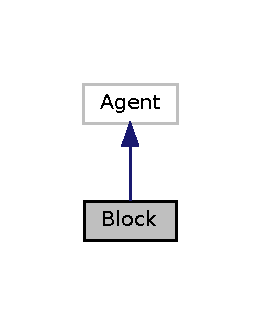
\includegraphics[width=125pt]{classBlock__inherit__graph}
\end{center}
\end{figure}


Collaboration diagram for Block\+:
\nopagebreak
\begin{figure}[H]
\begin{center}
\leavevmode
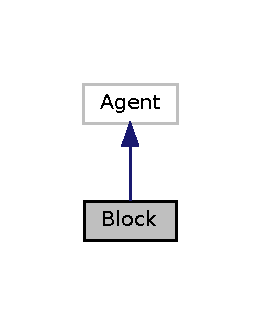
\includegraphics[width=125pt]{classBlock__coll__graph}
\end{center}
\end{figure}
\subsection*{Public Member Functions}
\begin{DoxyCompactItemize}
\item 
\mbox{\Hypertarget{classBlock_a8ac530339fd0753127baba8a1403e2d1}\label{classBlock_a8ac530339fd0753127baba8a1403e2d1}} 
{\bfseries Block} (json spec, World \&world)
\end{DoxyCompactItemize}


The documentation for this class was generated from the following file\+:\begin{DoxyCompactItemize}
\item 
block.\+h\end{DoxyCompactItemize}

\hypertarget{classBlockController}{}\section{Block\+Controller Class Reference}
\label{classBlockController}\index{Block\+Controller@{Block\+Controller}}


Inheritance diagram for Block\+Controller\+:
\nopagebreak
\begin{figure}[H]
\begin{center}
\leavevmode
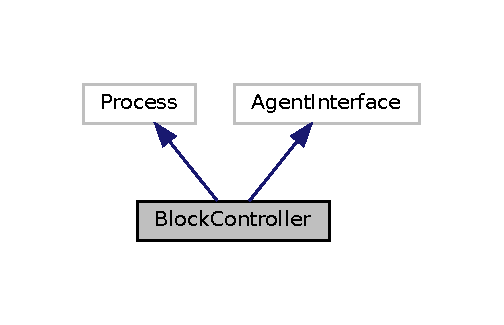
\includegraphics[width=242pt]{classBlockController__inherit__graph}
\end{center}
\end{figure}


Collaboration diagram for Block\+Controller\+:
\nopagebreak
\begin{figure}[H]
\begin{center}
\leavevmode
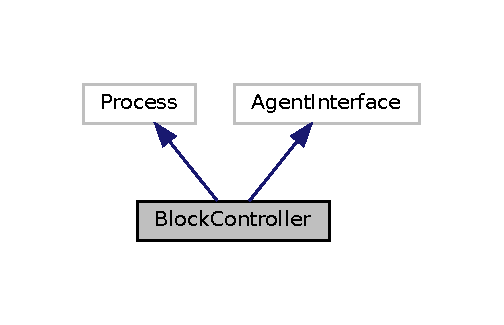
\includegraphics[width=242pt]{classBlockController__coll__graph}
\end{center}
\end{figure}
\subsection*{Public Member Functions}
\begin{DoxyCompactItemize}
\item 
\mbox{\Hypertarget{classBlockController_a5fab6bbac43e43d35debc69fba15e08a}\label{classBlockController_a5fab6bbac43e43d35debc69fba15e08a}} 
void {\bfseries init} ()
\item 
\mbox{\Hypertarget{classBlockController_ad75ee01c90b8892462199ea68b0541c3}\label{classBlockController_ad75ee01c90b8892462199ea68b0541c3}} 
void {\bfseries start} ()
\item 
\mbox{\Hypertarget{classBlockController_a244582d5298910da92b770b1a4811c82}\label{classBlockController_a244582d5298910da92b770b1a4811c82}} 
void {\bfseries update} ()
\item 
\mbox{\Hypertarget{classBlockController_a7ce9687c907f0d1bb99cccbef26cc26a}\label{classBlockController_a7ce9687c907f0d1bb99cccbef26cc26a}} 
void {\bfseries stop} ()
\end{DoxyCompactItemize}


The documentation for this class was generated from the following file\+:\begin{DoxyCompactItemize}
\item 
block.\+h\end{DoxyCompactItemize}

\hypertarget{classCoordinator}{}\section{Coordinator Class Reference}
\label{classCoordinator}\index{Coordinator@{Coordinator}}


Inheritance diagram for Coordinator\+:
\nopagebreak
\begin{figure}[H]
\begin{center}
\leavevmode
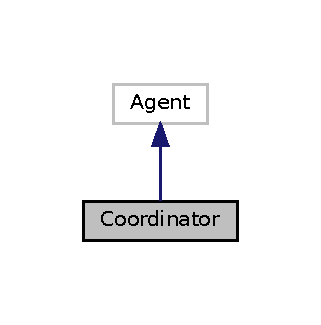
\includegraphics[width=154pt]{classCoordinator__inherit__graph}
\end{center}
\end{figure}


Collaboration diagram for Coordinator\+:
\nopagebreak
\begin{figure}[H]
\begin{center}
\leavevmode
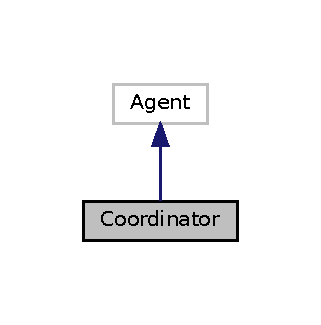
\includegraphics[width=154pt]{classCoordinator__coll__graph}
\end{center}
\end{figure}
\subsection*{Public Member Functions}
\begin{DoxyCompactItemize}
\item 
\mbox{\Hypertarget{classCoordinator_ab85d4c76f4356c066eaba655c0533c23}\label{classCoordinator_ab85d4c76f4356c066eaba655c0533c23}} 
{\bfseries Coordinator} (json spec, World \&world)
\end{DoxyCompactItemize}


The documentation for this class was generated from the following file\+:\begin{DoxyCompactItemize}
\item 
coordinator.\+h\end{DoxyCompactItemize}

\hypertarget{classCoordinatorController}{}\section{Coordinator\+Controller Class Reference}
\label{classCoordinatorController}\index{Coordinator\+Controller@{Coordinator\+Controller}}


Inheritance diagram for Coordinator\+Controller\+:
\nopagebreak
\begin{figure}[H]
\begin{center}
\leavevmode
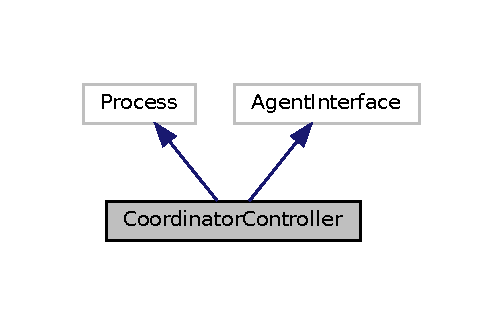
\includegraphics[width=242pt]{classCoordinatorController__inherit__graph}
\end{center}
\end{figure}


Collaboration diagram for Coordinator\+Controller\+:
\nopagebreak
\begin{figure}[H]
\begin{center}
\leavevmode
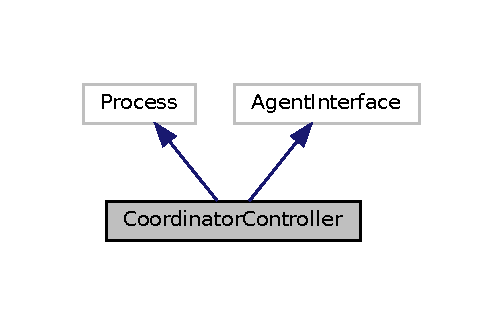
\includegraphics[width=242pt]{classCoordinatorController__coll__graph}
\end{center}
\end{figure}
\subsection*{Public Member Functions}
\begin{DoxyCompactItemize}
\item 
\mbox{\Hypertarget{classCoordinatorController_aadbb6ec1adad8359b9898590af18b7ff}\label{classCoordinatorController_aadbb6ec1adad8359b9898590af18b7ff}} 
void {\bfseries init} ()
\item 
\mbox{\Hypertarget{classCoordinatorController_a5b0e4d28b82a953cba030a90e5412c3a}\label{classCoordinatorController_a5b0e4d28b82a953cba030a90e5412c3a}} 
void {\bfseries start} ()
\item 
\mbox{\Hypertarget{classCoordinatorController_ac4a102259abb9389dbe84d1f22909e92}\label{classCoordinatorController_ac4a102259abb9389dbe84d1f22909e92}} 
void {\bfseries update} ()
\item 
\mbox{\Hypertarget{classCoordinatorController_ae69ecb3b5074de75c1753d6f188ba1c2}\label{classCoordinatorController_ae69ecb3b5074de75c1753d6f188ba1c2}} 
void {\bfseries stop} ()
\end{DoxyCompactItemize}


The documentation for this class was generated from the following file\+:\begin{DoxyCompactItemize}
\item 
coordinator.\+h\end{DoxyCompactItemize}

\hypertarget{classFinish}{}\section{Finish Class Reference}
\label{classFinish}\index{Finish@{Finish}}


Inheritance diagram for Finish\+:
\nopagebreak
\begin{figure}[H]
\begin{center}
\leavevmode
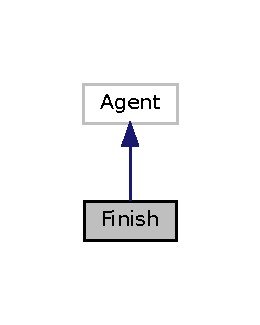
\includegraphics[width=125pt]{classFinish__inherit__graph}
\end{center}
\end{figure}


Collaboration diagram for Finish\+:
\nopagebreak
\begin{figure}[H]
\begin{center}
\leavevmode
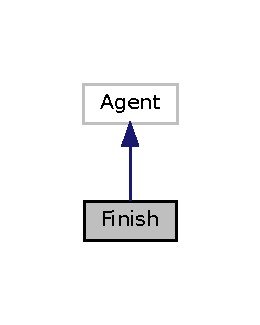
\includegraphics[width=125pt]{classFinish__coll__graph}
\end{center}
\end{figure}
\subsection*{Public Member Functions}
\begin{DoxyCompactItemize}
\item 
\mbox{\Hypertarget{classFinish_a22401ebe02f7822a86048e25e95114e8}\label{classFinish_a22401ebe02f7822a86048e25e95114e8}} 
{\bfseries Finish} (json spec, World \&world)
\end{DoxyCompactItemize}


The documentation for this class was generated from the following file\+:\begin{DoxyCompactItemize}
\item 
finish.\+h\end{DoxyCompactItemize}

\hypertarget{classFinishController}{}\section{Finish\+Controller Class Reference}
\label{classFinishController}\index{Finish\+Controller@{Finish\+Controller}}


Inheritance diagram for Finish\+Controller\+:
\nopagebreak
\begin{figure}[H]
\begin{center}
\leavevmode
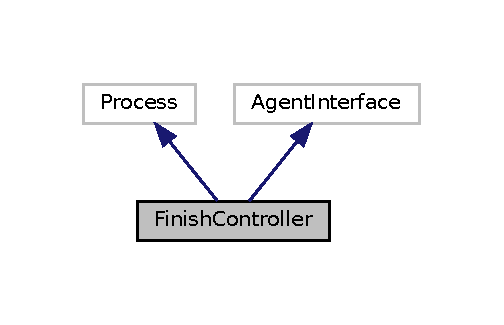
\includegraphics[width=242pt]{classFinishController__inherit__graph}
\end{center}
\end{figure}


Collaboration diagram for Finish\+Controller\+:
\nopagebreak
\begin{figure}[H]
\begin{center}
\leavevmode
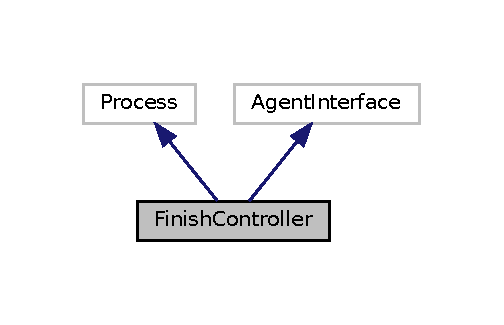
\includegraphics[width=242pt]{classFinishController__coll__graph}
\end{center}
\end{figure}
\subsection*{Public Member Functions}
\begin{DoxyCompactItemize}
\item 
\mbox{\Hypertarget{classFinishController_a5c2b92cc1d7f9000c36a3b28dab2dab2}\label{classFinishController_a5c2b92cc1d7f9000c36a3b28dab2dab2}} 
void {\bfseries init} ()
\item 
\mbox{\Hypertarget{classFinishController_a7c92091d8eb58f50d403f127956ae339}\label{classFinishController_a7c92091d8eb58f50d403f127956ae339}} 
void {\bfseries start} ()
\item 
\mbox{\Hypertarget{classFinishController_ace9a0d5687e3c2f8ea48dd0d9f5930da}\label{classFinishController_ace9a0d5687e3c2f8ea48dd0d9f5930da}} 
void {\bfseries update} ()
\item 
\mbox{\Hypertarget{classFinishController_abffc1d3517f007806404a491cfd2cb46}\label{classFinishController_abffc1d3517f007806404a491cfd2cb46}} 
void {\bfseries stop} ()
\end{DoxyCompactItemize}


The documentation for this class was generated from the following file\+:\begin{DoxyCompactItemize}
\item 
finish.\+h\end{DoxyCompactItemize}

\hypertarget{classMazeGenerator}{}\section{Maze\+Generator Class Reference}
\label{classMazeGenerator}\index{Maze\+Generator@{Maze\+Generator}}


Generates Random Maze.  




{\ttfamily \#include $<$mazegenerator.\+h$>$}

\subsection*{Public Member Functions}
\begin{DoxyCompactItemize}
\item 
void \hyperlink{classMazeGenerator_a67dbf663cdcc539fdb7583e8adcd58dc}{generate\+\_\+maze} (std\+::pair$<$ double, double $>$ location)
\begin{DoxyCompactList}\small\item\em Generates a random maze. \end{DoxyCompactList}\item 
const std\+::vector$<$ std\+::pair$<$ double, double $>$ $>$ \hyperlink{classMazeGenerator_ad3273f40be7ddb219fb419a8c0d707c3}{get\+\_\+walls} ()
\begin{DoxyCompactList}\small\item\em Generates vector of coordinates for walls to generate. \end{DoxyCompactList}\item 
const std\+::pair$<$ double, double $>$ \hyperlink{classMazeGenerator_a98a262b1588845a44c47ff59f9f3dccd}{get\+\_\+finish} ()
\begin{DoxyCompactList}\small\item\em Gets finish line coordinate. \end{DoxyCompactList}\end{DoxyCompactItemize}


\subsection{Detailed Description}
Generates Random Maze. 

Maze generator randomly generates a random maze within a defined rectangle.~\newline
Note that at the moment, the size is static and implementation is crude.~\newline
To-\/do\+: Dynamically scale maze, add param for maze size, optimize finish line, 

\subsection{Member Function Documentation}
\mbox{\Hypertarget{classMazeGenerator_a67dbf663cdcc539fdb7583e8adcd58dc}\label{classMazeGenerator_a67dbf663cdcc539fdb7583e8adcd58dc}} 
\index{Maze\+Generator@{Maze\+Generator}!generate\+\_\+maze@{generate\+\_\+maze}}
\index{generate\+\_\+maze@{generate\+\_\+maze}!Maze\+Generator@{Maze\+Generator}}
\subsubsection{\texorpdfstring{generate\+\_\+maze()}{generate\_maze()}}
{\footnotesize\ttfamily void Maze\+Generator\+::generate\+\_\+maze (\begin{DoxyParamCaption}\item[{std\+::pair$<$ double, double $>$}]{location }\end{DoxyParamCaption})}



Generates a random maze. 

{\bfseries generate\+\_\+maze} returns coordinates for the walls of a randomly generated maze. Its input is the starting location for the generator. \mbox{\Hypertarget{classMazeGenerator_a98a262b1588845a44c47ff59f9f3dccd}\label{classMazeGenerator_a98a262b1588845a44c47ff59f9f3dccd}} 
\index{Maze\+Generator@{Maze\+Generator}!get\+\_\+finish@{get\+\_\+finish}}
\index{get\+\_\+finish@{get\+\_\+finish}!Maze\+Generator@{Maze\+Generator}}
\subsubsection{\texorpdfstring{get\+\_\+finish()}{get\_finish()}}
{\footnotesize\ttfamily const std\+::pair$<$ double, double $>$ Maze\+Generator\+::get\+\_\+finish (\begin{DoxyParamCaption}{ }\end{DoxyParamCaption})}



Gets finish line coordinate. 

Get finish checks the corners of the map for an open cell to place the finish line, which is just a custom agent.~\newline
 To-\/do\+: Make smarter and randomize, incorporate scaling and dynamic map size \mbox{\Hypertarget{classMazeGenerator_ad3273f40be7ddb219fb419a8c0d707c3}\label{classMazeGenerator_ad3273f40be7ddb219fb419a8c0d707c3}} 
\index{Maze\+Generator@{Maze\+Generator}!get\+\_\+walls@{get\+\_\+walls}}
\index{get\+\_\+walls@{get\+\_\+walls}!Maze\+Generator@{Maze\+Generator}}
\subsubsection{\texorpdfstring{get\+\_\+walls()}{get\_walls()}}
{\footnotesize\ttfamily const std\+::vector$<$ std\+::pair$<$ double, double $>$ $>$ Maze\+Generator\+::get\+\_\+walls (\begin{DoxyParamCaption}{ }\end{DoxyParamCaption})}



Generates vector of coordinates for walls to generate. 

{\bfseries get\+\_\+walls} generates coordinates for walls by removing the visited coordinates from all possible coordinates. 

The documentation for this class was generated from the following file\+:\begin{DoxyCompactItemize}
\item 
mazegenerator.\+h\end{DoxyCompactItemize}

\hypertarget{classWanderer}{}\section{Wanderer Class Reference}
\label{classWanderer}\index{Wanderer@{Wanderer}}


Inheritance diagram for Wanderer\+:
\nopagebreak
\begin{figure}[H]
\begin{center}
\leavevmode
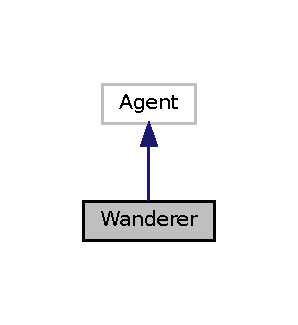
\includegraphics[width=143pt]{classWanderer__inherit__graph}
\end{center}
\end{figure}


Collaboration diagram for Wanderer\+:
\nopagebreak
\begin{figure}[H]
\begin{center}
\leavevmode
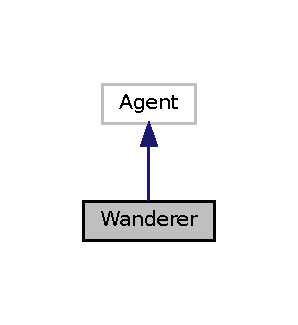
\includegraphics[width=143pt]{classWanderer__coll__graph}
\end{center}
\end{figure}
\subsection*{Public Member Functions}
\begin{DoxyCompactItemize}
\item 
\mbox{\Hypertarget{classWanderer_ac1c59ca77b69786ca6717707e5e07344}\label{classWanderer_ac1c59ca77b69786ca6717707e5e07344}} 
{\bfseries Wanderer} (json spec, World \&world)
\end{DoxyCompactItemize}


The documentation for this class was generated from the following file\+:\begin{DoxyCompactItemize}
\item 
wanderer.\+h\end{DoxyCompactItemize}

\hypertarget{classWandererController}{}\section{Wanderer\+Controller Class Reference}
\label{classWandererController}\index{Wanderer\+Controller@{Wanderer\+Controller}}


Inheritance diagram for Wanderer\+Controller\+:
\nopagebreak
\begin{figure}[H]
\begin{center}
\leavevmode
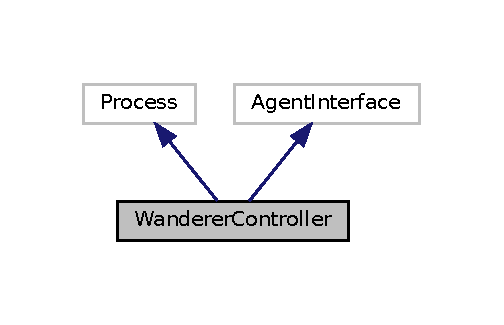
\includegraphics[width=242pt]{classWandererController__inherit__graph}
\end{center}
\end{figure}


Collaboration diagram for Wanderer\+Controller\+:
\nopagebreak
\begin{figure}[H]
\begin{center}
\leavevmode
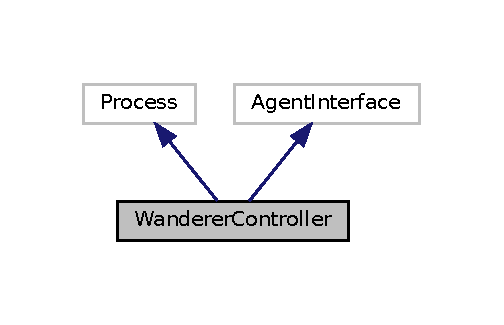
\includegraphics[width=242pt]{classWandererController__coll__graph}
\end{center}
\end{figure}
\subsection*{Public Member Functions}
\begin{DoxyCompactItemize}
\item 
\mbox{\Hypertarget{classWandererController_a602fa46c6de3bc7d1bd75f4cd6f6da84}\label{classWandererController_a602fa46c6de3bc7d1bd75f4cd6f6da84}} 
void {\bfseries init} ()
\item 
\mbox{\Hypertarget{classWandererController_a8f1816ff2b3d3cab4a783406fd0dcb3f}\label{classWandererController_a8f1816ff2b3d3cab4a783406fd0dcb3f}} 
void {\bfseries start} ()
\item 
\mbox{\Hypertarget{classWandererController_ad67334a5bf938e5d7f85a30ed27aea6a}\label{classWandererController_ad67334a5bf938e5d7f85a30ed27aea6a}} 
void {\bfseries update} ()
\item 
\mbox{\Hypertarget{classWandererController_adbea5e2c52606bcc2eecf485edb72e65}\label{classWandererController_adbea5e2c52606bcc2eecf485edb72e65}} 
void {\bfseries stop} ()
\end{DoxyCompactItemize}


The documentation for this class was generated from the following files\+:\begin{DoxyCompactItemize}
\item 
wanderer.\+h\item 
wanderer.\+cc\end{DoxyCompactItemize}

%--- End generated contents ---

% Index
\backmatter
\newpage
\phantomsection
\clearemptydoublepage
\addcontentsline{toc}{chapter}{Index}
\printindex

\end{document}
